\documentclass[tikz,border=2pt]{standalone}
\usepackage{amsmath,amssymb}
\usepackage{pgfplots}
\pgfplotsset{compat=1.18}
\usetikzlibrary{calc}

\begin{document}
% The support is where the probability lives: the isolated points of a discrete pmf, or the
% set where a density is positive (here [0, infinity) for the exponential distribution).
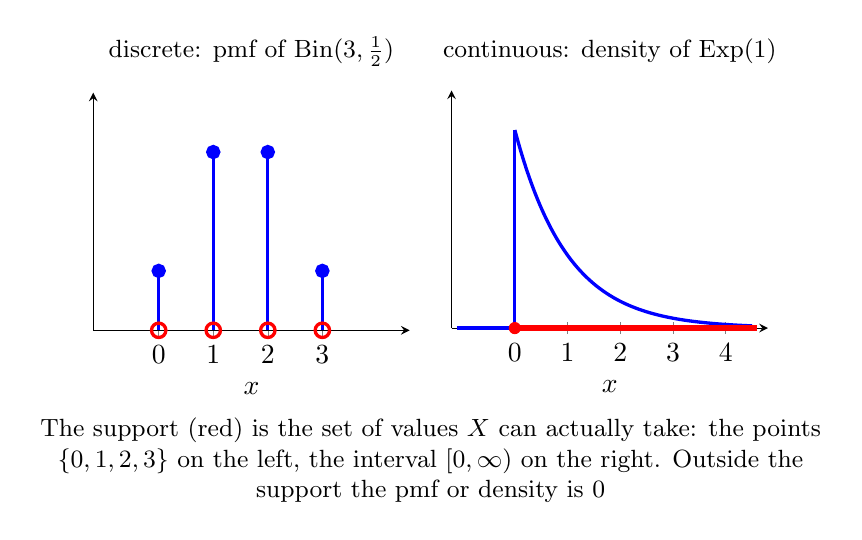
\begin{tikzpicture}
	\begin{axis}[
		name=p1, axis lines=left, xmin=-1.2, xmax=4.6, ymin=0, ymax=0.5,
		xtick={0,1,2,3}, ytick=\empty,
		xlabel={$x$},
		width=5.6cm, height=4.6cm, clip=false, title={discrete: pmf of $\operatorname{Bin}(3,\tfrac12)$}, title style={font=\small}
		]
		\addplot[ycomb, blue, very thick, mark=*, mark size=2pt] coordinates {(0,0.125) (1,0.375) (2,0.375) (3,0.125)};
		\draw[red, very thick] (axis cs:0,0) circle (2.6pt);
		\draw[red, very thick] (axis cs:1,0) circle (2.6pt);
		\draw[red, very thick] (axis cs:2,0) circle (2.6pt);
		\draw[red, very thick] (axis cs:3,0) circle (2.6pt);
	\end{axis}
	\begin{axis}[
		name=p2, at={(p1.outer east)}, anchor=outer west, xshift=3mm,
		axis lines=left, xmin=-1.2, xmax=4.8, ymin=0, ymax=1.2,
		xtick={0,1,2,3,4}, ytick=\empty,
		xlabel={$x$},
		samples=120, smooth, width=5.6cm, height=4.6cm, clip=false, title={continuous: density of $\operatorname{Exp}(1)$}, title style={font=\small}
		]
		\draw[blue, very thick] (axis cs:-1.1,0) -- (axis cs:0,0);
		\addplot[blue, very thick, domain=0:4.5] {exp(-x)};
		\draw[blue, very thick] (axis cs:0,0) -- (axis cs:0,1);
		\draw[red, line width=2pt] (axis cs:0,0) -- (axis cs:4.6,0);
		\fill[red] (axis cs:0,0) circle (2.2pt);
	\end{axis}
	\node[anchor=north, font=\small, align=flush center, text width=10cm] at ([yshift=-2pt]$(p1.outer south)!0.5!(p2.outer south)$) {The support (red) is the set of values $X$ can actually take: the points $\{0,1,2,3\}$ on the left, the interval $[0,\infty)$ on the right. Outside the support the pmf or density is $0$};
\end{tikzpicture}
\end{document}
